\section{Illustrative Evaluation}
\label{sec:evaluation}
This section reports model outputs only. The labels ``materialized'' and ``tiled'' name the schedules in Equation~\ref{eq:bytes}; they do not name measured libraries. No device, batch execution, warmup procedure, or timing instrument was used. The figures should therefore be read as explanations of the model rather than as comparative performance evidence for an implementation.

\subsection{Sequence-length scaling}
Figure~\ref{fig:time} plots the baseline predicted time at $d=64$. At small sequence lengths, the fixed launch term occupies a substantial portion of both totals. Reducing the transfer term then changes only a small fraction of the visible time. As the workload grows, the quadratic components become more influential, and the schedules separate. The separation is a consequence of the assigned coefficients, not a discovery about an actual GPU.

\begin{figure}[t]
 \centering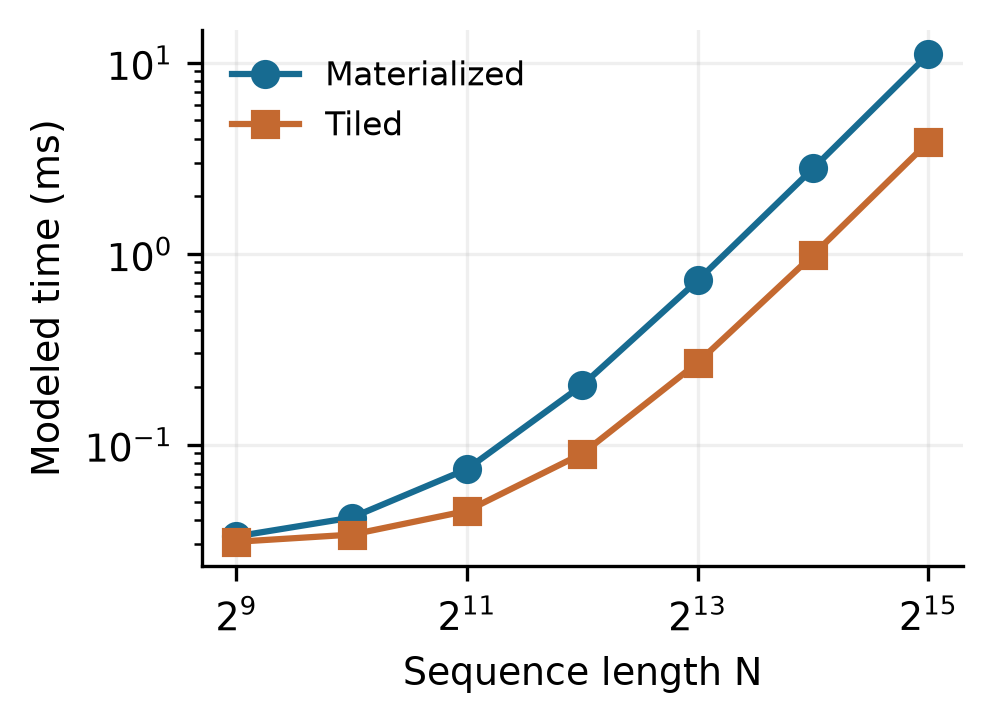
\includegraphics[width=\linewidth]{assets/runtime.png}
 \caption{Synthetic forward-time model at $d=64$. The log axes expose both the launch-dominated region and the larger-workload trend. No hardware measurements are plotted.}
 \label{fig:time}
\end{figure}

An important diagnostic is to inspect the selected component, not only the total. In the materialized schedule, the byte term can dominate while the tiled schedule is limited by arithmetic. In that regime, adding bandwidth to the tiled case provides little benefit within the model. A report that simply attributes every improvement to ``faster memory'' would miss the change in the active constraint.

Table~\ref{tab:results} gives a subset of generated values. Times are rounded for readability, whereas ratios are computed from unrounded model outputs. The table is generated programmatically and is deliberately small: its role is to provide numerical anchors for the curves, not to duplicate every record in the CSV. The full dataset remains available for inspection.

\begin{table}[t]
\caption{Deterministic illustrative outputs for $d=64$. Times include the assumed 30~$\mu$s overhead; these are not measurements.}
\label{tab:results}
\centering
\begin{tabular}{rrrr}
\toprule
$N$ & Materialized (ms) & Tiled (ms) & Ratio \\
\midrule
512 & 0.033 & 0.031 & 1.07 \\
1024 & 0.041 & 0.034 & 1.23 \\
2048 & 0.074 & 0.045 & 1.66 \\
4096 & 0.205 & 0.090 & 2.28 \\
8192 & 0.724 & 0.269 & 2.69 \\
16384 & 2.794 & 0.984 & 2.84 \\
32768 & 11.064 & 3.848 & 2.88 \\
\bottomrule
\end{tabular}
\end{table}


\subsection{Temporary workspace}
Figure~\ref{fig:workspace} uses the separately defined workspace expressions. The materialized curve grows quadratically in $N$, while the tiled expression combines a linear component with a fixed tile term. At smaller shapes, that fixed term matters; at larger shapes, the difference in growth rates becomes the dominant feature. This is a statement about the allocation model, not a measured maximum from a memory profiler.

\begin{figure}[t]
 \centering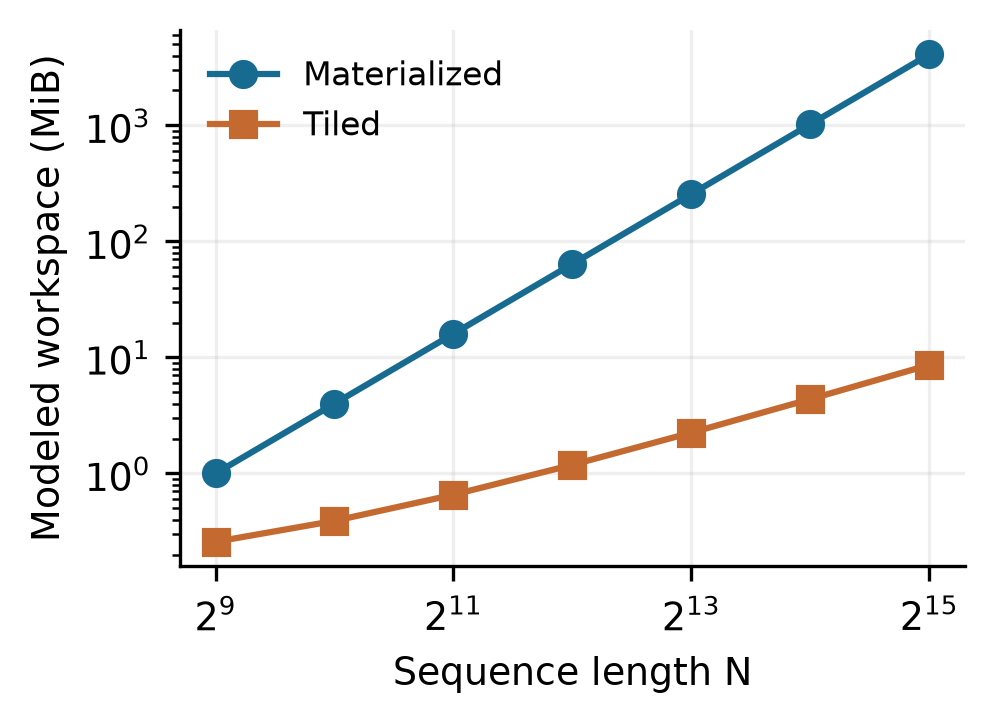
\includegraphics[width=\linewidth]{assets/workspace.png}
 \caption{Synthetic temporary workspace. Inputs, model weights, allocator overhead, and backward state are excluded from both curves. Binary MiB units are used.}
 \label{fig:workspace}
\end{figure}

It would be inappropriate to turn this plot directly into an out-of-memory threshold for a named device. Such a threshold requires a complete accounting of persistent tensors, batch size, framework allocations, and reserve capacity. It also requires the actual allocation policy. Fragmentation or an implementation-specific temporary can change feasibility even when the leading expression remains favorable. The plot instead identifies why a measured study should record peak allocation separately from transferred bytes.

\subsection{The head-dimension dimension}
Figure~\ref{fig:heatmap} expands the comparison across head dimensions. Increasing $d$ raises the shared arithmetic count and the linear traffic terms, while the quadratic traffic difference remains fixed by our coefficients. Consequently, the relative contribution of the traffic reduction changes. A single baseline head dimension cannot represent the whole parameter space even in this simplified setting.

\begin{figure*}[t]
 \centering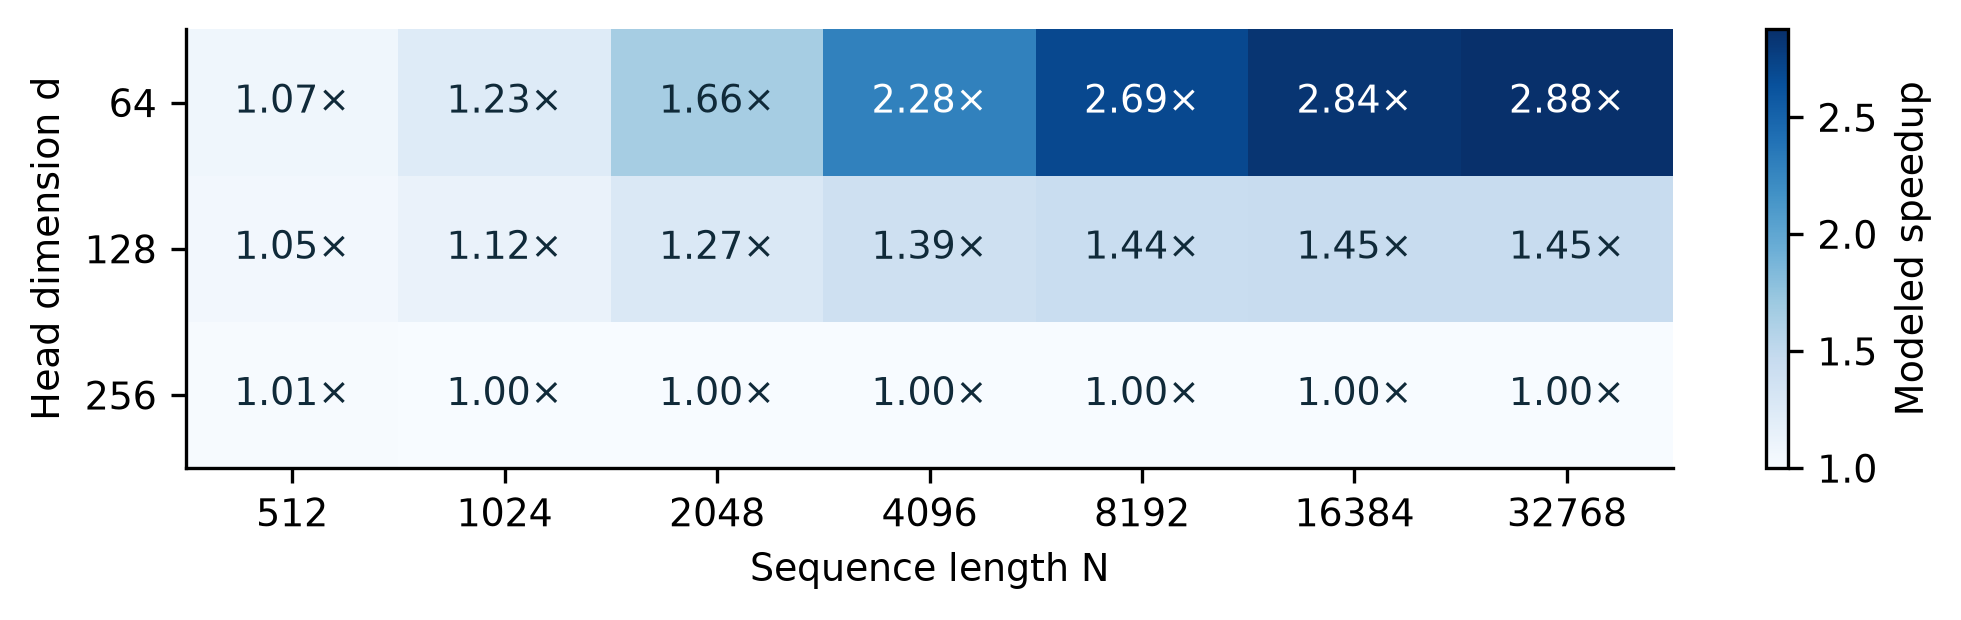
\includegraphics[width=.86\textwidth]{assets/speedup-grid.png}
 \caption{Synthetic speedup across sequence lengths and head dimensions. Each cell is a deterministic ratio from the same model; the colors are not evidence of measurement uncertainty or statistical significance.}
 \label{fig:heatmap}
\end{figure*}

This observation suggests a reporting rule for real studies: shapes should be treated as part of the workload definition, not as incidental benchmark settings. Reporting only the best-performing shape can make an optimization appear more general than the evidence supports. A useful shape sweep includes cases where the improvement is small, as these cases often reveal the limiting mechanism most clearly.

\subsection{Reading a speedup responsibly}
A ratio can obscure the absolute scale of a benefit. A large percentage change on a tiny operation may have little practical effect, while a moderate ratio on a dominant operation can matter greatly. We therefore pair the ratio grid with an absolute-time plot and a workspace plot. Their agreement is not guaranteed; when they tell different stories, the difference is informative.

The model also illustrates why a numerical comparison should not be labeled a benchmark merely because it has axes, legends, and units. The artifact contains a reproducible calculation, but reproducibility alone does not establish empirical validity. All performance language in this section is conditional: it describes what the chosen model predicts, and it identifies what a subsequent experiment would need to test.
